\documentclass[../custom]{flashcards}
\usepackage{amsmath}
\usepackage{booktabs}
\usepackage{array}
\usepackage{enumitem}
\usepackage{tikz}
\usepackage{float}

\newcommand{\studyArea}{Behavioral Finance}

\def\labelitemii{$\circ$}
\def\labelitemiii{$\diamond$}
\def\labelitemiv{$\cdot$}

\begin{document}
\cardfrontstyle{headings}
\cardfrontfoot{Study Session 3}

\begin{flashcard}[\studyArea]{Micro and Macro Behavioral Finance}
    \begin{itemize}
        \item \textbf{Micro behavioral finance} describes the decision-making process of individuals. It tries to explain why they deviate from traditional finance.
        \item \textbf{Macro behavioral finance} tries to explain how and why markets deviate from the efficiency of traditional finance. 
    \end{itemize}
\end{flashcard}

\begin{flashcard}[\studyArea]{Four Axioms of Rational Decision Makers}
    \begin{itemize}
        \item \textbf{Completeness.} Given a choice between $A$ and $B$, either $A$ or $B$ is preferred, or indifference.
        \item \textbf{Transitivity.} If $A$ is preferred to $B$ is preferred to $C$ then $A$ must be preferred to $C$.
        \item \textbf{Independence.} If $A$ and $B$ are mutually exclusive with $A$ preferred, and $C$ is an additional choice that adds positive utility, then $A + \alpha C$ is preferred to $B + \alpha C$. Here $\alpha C$ is some portion of $C$.
        \item \textbf{Continuity.} If $A$ is preferred to $B$ is preferred to $C$, then there will be a combination of $A$ and $C$ indifferent from $B$.
    \end{itemize}
\end{flashcard}

\begin{flashcard}[\studyArea]{Bayes' Formula}
    \begin{flushleft}
        \begin{align*}
            P(A \vert B) &= \frac{P(B \vert A)}{P(B)} P(A)\\
            \\
            \text{where:}\\
            P(A \vert B) &= \text{probability of $A$ occurring given that $B$ has occurred}\\
            P(B \vert A) &= \text{probability of $B$ occurring given that $A$ has occurred}\\
            P(A) &= \text{probability of $A$ occurring}\\
            P(B) &= \text{probability of $B$ occurring}
        \end{align*}
    \end{flushleft}
\end{flashcard}

\begin{flashcard}[\studyArea]{Risk Aversion in Behavioral Finance}
    \begin{flushleft}
        Traditional finance assumes individuals are risk-averse and prefer greater certainty over less certainty. Behavioral finance uses the following categories.
        \begin{itemize}
            \item \textbf{Risk-averse} have a greater loss of utility for a given loss of wealth than they gain in utility for the same risk in wealth.
            \item \textbf{Risk-neutral} gains or loses the same amount of utility for a given gain or loss of wealth.
            \item \textbf{Risk seeker} gains more utility for a rise in wealth than they lose in an equivalent loss of wealth.
        \end{itemize}
    \end{flushleft}
\end{flashcard}

\begin{flashcard}[\studyArea]{Traditional and Behavioral Finance Utility Functions}
    \begin{itemize}
        \item Traditional finance is based in utility theory with an assumption of diminishing marginal return. This implies
            \begin{itemize}
                \item The risk-averse utility function is concave. As more wealth is added, utility increases at a diminishing rate.
                \item Convex indifference curves due to diminishing marginal rates of substitution.
            \end{itemize}
        \item Behavioral finance observes people who are both risk-seeking and risk-averse. This can lead to complex, double-inflection utility functions.
    \end{itemize}
\end{flashcard}

\begin{flashcard}[\studyArea]{Bounded Rationality}
    \begin{flushleft}
        Bounded rationality assumes a maximum capacity of knowledge. It removes assumptions of perfect information, rational decision marking, and consistent utility maximization. Instead, outcomes that offer sufficient satisfaction, but not optimal utility are sufficient.
    \end{flushleft}
\end{flashcard}

\begin{flashcard}[\studyArea]{Two Phases of Prospect Theory}
    \begin{itemize}
        \item \textbf{Editing phase.} Economically identical outcomes are grouped, and a reference point is established to rank proposals. This simplifies the number of choices before the decision phase. There is a risk that the reference point frames the proposal as a gain or loss, affecting the decision phase.
        \item \textbf{Decision phase.} Investors focus on loss aversion rather than risk aversion. I.e., they are concerned more with the change in wealth rather than the resulting level of wealth. Also, there is a larger utility decrease for losses than gains of the same amount. Investors tend to fear losses and become risk seeking in attempt to avoid them.
    \end{itemize}
\end{flashcard}

\begin{flashcard}[\studyArea]{Editing Phase of Prospect Theory}
    \begin{enumerate}
        \item \textbf{Codification} codes the proposal as a gain or loss, and assigns a probability to each outcome using a selected reference point.
        \item \textbf{Combination} simplifies outcomes by combining those with identical values.
        \item \textbf{Segregation} separates expected return into risky and risk-free components.
        \item \textbf{Cancellation} removes outcomes common to two proposals.
        \item \textbf{Simplification} applies to very small differences in probabilities or very unlikely outcomes.
        \item \textbf{Detection of dominance} discards any proposal that is clearly dominated by another.
    \end{enumerate}
\end{flashcard}

\begin{flashcard}[\studyArea]{Evaluation Phase of Prospect Theory}
    \begin{flushleft}
        In the evaluation phase, investors place values on outcomes and probability-weight them to determine expected utility. The implications are
        \begin{itemize}
            \item Individuals overreact to small probabilities and underreact to large probabilities.
            \item The value function is S-shaped and asymmetric with larger declines in value for losses than rises for corresponding gains.
            \item Thus, most investors are risk-averse when presented with gains, and risk seekers when confronted with likely losses.
            \item This could explain why investors focus on high- and low-risk investments, but not medium-risk investments.
        \end{itemize}
    \end{flushleft}
\end{flashcard}

\begin{flashcard}[\studyArea]{Comparison Between Traditional Finance and Bounded Rationality and Prospect Theory}
    \begin{tabular}
       {>{\raggedright}p{2.1in}
        >{\raggedright\arraybackslash}p{2.1in}} \toprule
        \textit{Traditional Finance Assumes:} &
        \textit{Bounded Rationality and Prospect Theory Assume:}\\ \midrule

        Unlimited perfect knowledge &
        Capacity limitations on knowledge\\ \addlinespace

        Utility maximization &
        Satisfice\\ \addlinespace

        Fully rational decision making &
        Cognitive limits on decision making\\ \addlinespace

        Risk aversion &
        Reference dependence to determine gain or loss leading to possible cognitive errors\\ \bottomrule
    \end{tabular}
\end{flashcard}

\begin{flashcard}[\studyArea]{Efficient Market Hypothesis}
    \begin{itemize}
        \item \textbf{Weak-form efficient} means current prices incorporate all past price and volume data. Can't generate excess return using technical analysis.
        \item \textbf{Semi-strong form efficient} means prices reflect all public information, including past price and volume data. As soon as information is released, it is fully and accurately reflected in prices. Can't generate excess returns using technical or fundamental analysis.
        \item \textbf{Strong-form efficient} means prices reflect all public and non-public information. No analysis based on inside or public information can generate excess returns. This is generally not accepted as nonpublic information is associated with excess returns.
    \end{itemize}
\end{flashcard}

\begin{flashcard}[\studyArea]{Support and Challenges to the Efficient Market Hypothesis}
    \begin{itemize}[nosep]
        \item Support for EMH
            \begin{itemize}[nosep]
                \item Historical studies show almost zero correlation between past and current prices. This is consistent with weak-form EMH.
                \item Event studies look for evidence that certain events predict price movement. Studies about stock splits show rises in prices leading up to the split and complete an adjustment coincident with the split. This is consistent with semi-strong EMH.
                \item Studies of mutual fund managers show that the majority have negative alpha both before and after management fees. This is consistent with semi-strong EMH.
            \end{itemize}
        \item Challenges to EMH
            \begin{itemize}[nosep]
                \item Many studies show that value stocks with low P/E, P/B and P/S outperform growth stocks.
                \item Studies show abnormal positive return for small-cap stocks.
                \item Others suggest abnormal value stock returns are because of higher risk. Famma and French suggest including market cap and B/P in the CAPM model to adjust for this.
                \item Studies show moving averages and resistance and support levels can trigger buys and sells.
                \item Calendar anomalies show higher returns in January, the last day of the month, and the first four days of the month.
                \item Most technical anomalies should disappear after transaction costs.
            \end{itemize}
    \end{itemize}
\end{flashcard}

\begin{flashcard}[\studyArea]{Consumption and Savings Model}
    \begin{flushleft}
        Traditional finance assumes investors are able to save and invest in the early stages of life to fund retirement. This requires self control to delay short-term gratification.\newline

        The consumption and savings model suggests individuals use mental accounting and framing biases. They mentally account wealth as current income, assets owned, and present value of future income. They are less likely to spend from current assets and expected future wages.\newline

        This can lead to framing biases. E.g., if a bonus is viewed as current income instead of future income, one is more likely to spend it.
    \end{flushleft}
\end{flashcard}

\begin{flashcard}[\studyArea]{Behavioral Asset Pricing Model}
    \begin{flushleft}
        Traditional asset pricing models determine prices through unbiased analysis of risk and return, discounting cash flows at a required return based on the risk-free rate.\newline

        The behavioral asset pricing model adds a sentiment premium to the discount rate, making required return the sum of the risk-free rate, a risk premium, and a sentiment premium. The sentiment premium can be estimated by looking at the dispersion of analyst forecasts. Higher dispersion indicates a higher sentiment premium.
    \end{flushleft}
\end{flashcard}

\begin{flashcard}[\studyArea]{Behavioral Portfolio Theory}
    \begin{flushleft}
        Individuals construct portfolios by layers, with each layer having a different expected return and risk. Further, holdings are concentrated in nearly risk-free or high-risk assets. Layers are determined by
        \begin{itemize}
            \item The importance of the goal to the investor. Goals requiring high returns or low risk will get allocated accordingly.
            \item Asset selection is done by layer and based on the goal for that layer.
            \item The number of assets in a layer reflect risk aversion. Risk-averse investors will have more assets in each layer.
            \item If an investor believes he has an information advantage, more concentrated positions will be held.
            \item If an investor is loss-averse, he will have larger cash positions to avoid selling assets at a loss to meet liquidity needs.
        \end{itemize}
        The resulting portfolio appears diverse, but is likely suboptimal because the correlation between layers wasn't considered.
    \end{flushleft}
\end{flashcard}

\begin{flashcard}[\studyArea]{Adaptive Markets Hypothesis Model}
    \begin{flushleft}
        The AMH assumes market participants use heuristics until they stop working, and then adjust them. AMH assumes investors satisfice rather than maximize utility. They make decisions to reach subgoals based on information that they feel is sufficient. The AMH has the following conclusions
        \begin{itemize}
            \item The relationship of risk and return should not be stable. The market risk premium changes over time as the competitive environment changes.
            \item Active management can find opportunities to exploit arbitrage.
            \item No strategy will work all the time.
            \item Adaption and innovation are needed for continued success.
            \item Survivors change and adapt.
        \end{itemize}
    \end{flushleft}
\end{flashcard}

\begin{flashcard}[\studyArea]{Conservatism Bias}
    \begin{flushleft}
        Occurs when people hold on to a prior view or opinion and fail to consider new information. They overweight the initial probabilities and do not adjust probabilities for the new information.\newline

        May produce market participants who
        \begin{itemize}
            \item Are unwilling to update a view and therefore hold an investment too long.
            \item Hold an investment too long to avoid the mental effort of updating a view.
        \end{itemize}
    \end{flushleft}
\end{flashcard}

\begin{flashcard}[\studyArea]{Confirmation Bias}
    \begin{flushleft}
        Occurs when people look for new information or distort information to support an existing view. It's a kind of selection bias.\newline

        May produce market participants who
        \begin{itemize}
            \item Consider positive but ignore negative information, causing them to hold investments too long.
            \item Set up data screens or the decision process incorrectly to find what they want to see.
            \item Under-diversify as they become convinced their ideas are correct.
            \item Over-concentrate in their employer's stock believing they have an information advantage.
        \end{itemize}
    \end{flushleft}
\end{flashcard}

\begin{flashcard}[\studyArea]{Representativeness Bias}
    \begin{flushleft}
        \begin{itemize}
            \item Might rely on an overly simplistic past classification to categorize new information.
            \item In base-rate neglect, new information is given too much importance, taken to represent too much, and underlying probabilities are not sufficiently considered.
            \item In sample-size neglect, new information is overweighted without considering that the data is only a sample.\newline
        \end{itemize}

        May produce market participants who
        \begin{itemize}
            \item Attach too much importance to new pieces of information and have excessive turnover.
            \item Make decisions based on simple rules of thumb without more analysis, attaching either too much or too little importance to new information.
        \end{itemize}
    \end{flushleft}
\end{flashcard}

\begin{flashcard}[\studyArea]{Illusion of Control Bias}
    \begin{flushleft}
        The believe that people can control or affect outcomes. Often associated with emotional biases illusion or knowledge, self-attribution, and overconfidence biases.\newline

        May produce market participants who
        \begin{itemize}
            \item Trade more than is appropriate as they believe they can control the outcome of the trade.
            \item Fail to adequately diversify.
        \end{itemize}
    \end{flushleft}
\end{flashcard}

\begin{flashcard}[\studyArea]{Hindsight Bias}
    \begin{flushleft}
        Selective memory of past events or evaluation of what was knowable at the time. People tend to remember their correct views and forget their errors.\newline

        May produce market participants who
        \begin{itemize}
            \item Overestimate the rate at which they correctly predicted events, leading to an emotional overconfidence bias.
            \item Become overly critical of others' performance.
        \end{itemize}
    \end{flushleft}
\end{flashcard}

\begin{flashcard}[\studyArea]{Anchoring and Adjustment Bias}
    \begin{flushleft}
        Arises when people use psychological heuristic rules to unduly affect probabilities. When people estimate an unknown, they typically pick a value and adjust it with new information. New information is not dependent on initial estimates or starting points, and should be objectively considered without regard to the anchor point.\newline

        May produce market participants who
        \begin{itemize}
            \item Stay anchored to an initial estimate and do not adjust to new information.
        \end{itemize}
    \end{flushleft}
\end{flashcard}

\begin{flashcard}[\studyArea]{Mental Accounting Bias}
    \begin{flushleft}
Occurs when money is treated differently depending on how it is categorized. E.g., treating wages differently than a bonus for savings and investment purposes.\newline

        May produce market participants who
        \begin{itemize}
            \item Structure portfolios in layers to meet different goals.
            \item Fail to lower risk by adding assets with low correlation.
            \item Segregate return into arbitrary categories of income, realized gains, and unrealized gains. This tends to overemphasize income-generating assets.
        \end{itemize}
    \end{flushleft}
\end{flashcard}

\begin{flashcard}[\studyArea]{Framing Bias}
    \begin{flushleft}
        Occurs when the answer given is affected by the way the question is framed. E.g., being more likely to sell a stock at a particular price if the sale results in a gain.\newline

        May produce market participants who
        \begin{itemize}
            \item Fail to properly assess risk and end up overly risk-averse or risk-seeking.
            \item Choose suboptimal risk for their assets based on presentation.
            \item Become overly concerned with short term price movement and trade too often.
        \end{itemize}
    \end{flushleft}
\end{flashcard}

\begin{flashcard}[\studyArea]{Availability Bias}
    \begin{flushleft}
        Putting undue emphasis with information that is readily available. It can include
        \begin{itemize}
            \item Retrievability, focusing on what is first thought of.
            \item Categorization, putting emphasis on how an idea is categorized.
            \item Narrow range of experience.
            \item Resonance occurs when people assume what interest them is representative of what others find important.\newline
        \end{itemize}

        May produce market participants who
        \begin{itemize}
            \item Choose managers based on advertising.
            \item Limit investment choices to what they are familiar with leading to under-diversification and inappropriate asset allocation.
        \end{itemize}
    \end{flushleft}
\end{flashcard}

\begin{flashcard}[\studyArea]{Loss-Aversion Bias}
    \begin{flushleft}
        Arises from losing more utility from a loss than gaining utility from an equivalent gain.\newline

        May produce market participants who
        \begin{itemize}
            \item Hold on to losers too long and sell winners too quickly.
            \item Trade too often by selling for small gains, raising transaction costs.
            \item Incur too much risk by holding assets that have deteriorated in quality and lost value.
            \item Take excessive risk after a decline in the hopes of recovering.
            \item Allow framing of a reference point to determine if a position is a gain or loss.
            \item Treat money that is made on trades differently than other funds and taking excessive risk with such money.
            \item Overemphasize short-term potential losses resulting in a risk premium on stocks that is too high. This is called myopic loss aversion.
        \end{itemize}
    \end{flushleft}
\end{flashcard}

\begin{flashcard}[\studyArea]{Overconfidence Bias}
    \begin{flushleft}
        Leads people to overestimate their own intuitive ability or reasoning. Can show up as illusion of knowledge. Combined with self-attribution bias, people will take credit when things go right, but blame others for failure. Prediction overconfidence leads to underestimates of uncertainty and standard deviation of predictions. Certainty overconfidence is overstating the probability of being right.\newline

        May produce market participants who
        \begin{itemize}
            \item Underestimate risk and overestimate return.
            \item Under-diversify.
            \item Generate excessive turnover and transaction costs, resulting in lower returns.
        \end{itemize}
    \end{flushleft}
\end{flashcard}

\begin{flashcard}[\studyArea]{Self-Control Bias}
    \begin{flushleft}
        A failure to address long-term goals due to insufficient self-discipline.\newline

        May produce market participants who
        \begin{itemize}
            \item Have insufficient savings to fund retirement.
            \item Take excessive risk to try and compensate for insufficient savings.
            \item Overemphasize on income producing assets to meet short-term distribution needs.
        \end{itemize}
    \end{flushleft}
\end{flashcard}

\begin{flashcard}[\studyArea]{Status Quo Bias}
    \begin{flushleft}
        Based on an emotional desire to do nothing. If investment choices include the option to maintain existing choices, or if a choice will happen unless the investor opts out, status quo choices become more likely.\newline

        May produce market participants who
        \begin{itemize}
            \item Hold portfolios with inappropriate risk.
            \item Don't consider other, better investment options.
        \end{itemize}
    \end{flushleft}
\end{flashcard}

\begin{flashcard}[\studyArea]{Endowment Bias}
    \begin{flushleft}
        Keeping an investment for sentimental or otherwise investment-unrelated reason. E.g., a spouse holding on to their deceased spouse's investments, or having a maximum sale price higher than a maximum purchase price.\newline

        May produce market participants who
        \begin{itemize}
            \item Fail to sell an inappropriate asset resulting in inefficient allocations.
            \item Hold things they are familiar with because they provide a sense of comfort.
        \end{itemize}
    \end{flushleft}
\end{flashcard}

\begin{flashcard}[\studyArea]{Regret-Aversion Bias}
    \begin{flushleft}
        Occurs when people do nothing for fear that actions could be wrong. Their sense of regret is stronger for actions of commission as opposed to omission.\newline

        May produce market participants who
        \begin{itemize}
            \item Have excess conservatism because it's easier to see riskier assets underperform. This leads to long-term underperformance.
            \item Follow the consensus or popular opinion and tell themselves they are not to blame if others are wrong too. This is called herding behavior.
        \end{itemize}
    \end{flushleft}
\end{flashcard}

\begin{flashcard}[\studyArea]{Goals-Based Investing}
    \begin{itemize}
        \item Essential needs and obligations should be identified and quantified first. These should be met with low-risk investments as the base layer of the portfolio.
        \item Next is desired outcomes such as annual charity giving which can use medium-risk investments.
        \item Lastly low priority investments such as increasing the value of the portfolio for posthumous action can use higher-risk investments.
    \end{itemize}
\end{flashcard}

\begin{flashcard}[\studyArea]{Behaviorally Modified Asset Allocation}
    \begin{flushleft}
        BMAA works with clients to accommodate their cognitive and emotional biases. It starts with identifying an optimal portfolio using traditional finance. Then it considers the relative wealth and biases of the client to adjust that allocation.\newline

        \begin{itemize}
            \item High level of wealth versus lifestyle would be a low standard of living risk (SLR). Lower SLR allows deviation from an optimal portfolio.
            \item Biases that are cognitive in nature are easier to modify.
            \item Emotional biases are harder to modify and may have to be accommodated, resulting in a less efficient portfolio.
            \item The amount of deviation to accept from a traditional allocation should be established. Typically, this would use a range in which an asset is allowed to deviate.
        \end{itemize}
    \end{flushleft}
\end{flashcard}

\begin{flashcard}[\studyArea]{Barnewall Two-Way Behavioral Model}
    \begin{flushleft}
        Classifies investors as passive or active.
        \begin{itemize}
            \item \textbf{Passive investors} have not risked their own capital to gain wealth. E.g., disciplined saving or inheritance. They tend to be more risk-averse.
            \item \textbf{Active investors} risk their own capital to gain wealth and take an active role in investing their money. They are willing to give up security for control over their own wealth creation.
        \end{itemize}
    \end{flushleft}
\end{flashcard}

\begin{flashcard}[\studyArea]{Bailard, Biehl, and Kaiser Five-Way Behavioral Model}
    \begin{flushleft}
        Classifies investors along dimensions of confidence and method of action. Confidence measures level of confidence when making decisions and ranges from confident to anxious. Method of action measures decision making approach and ranges from careful to impetuous. BB\&K makes five categories using this grid.
        \begin{center}
            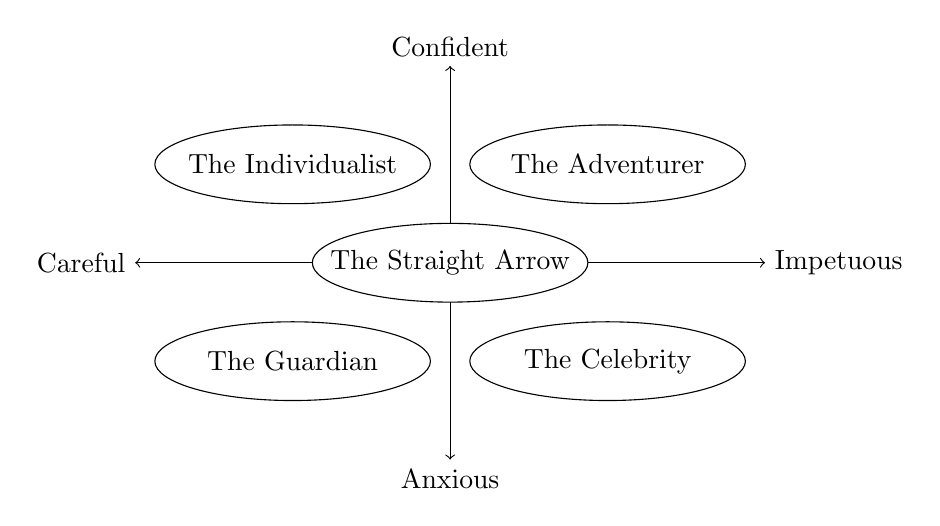
\begin{tikzpicture}
                \draw (0, 0) ellipse (1.75 and 0.5) node {The Straight Arrow};
                \draw (2, 1.25) ellipse (1.75 and 0.5) node {The Adventurer};
                \draw (-2, 1.25) ellipse (1.75 and 0.5) node {The Individualist};
                \draw (-2, -1.25) ellipse (1.75 and 0.5) node {The Guardian};
                \draw (2, -1.25) ellipse (1.75 and 0.5) node {The Celebrity};
                \draw[->] (-1.75, 0) -- (-4, 0) node[left] {Careful};
                \draw[->] (1.75, 0) -- (4, 0) node[right] {Impetuous};
                \draw[->] (0, 0.5) -- (0, 2.5) node[above] {Confident};
                \draw[->] (0, -0.5) -- (0, -2.5) node[below] {Anxious};
            \end{tikzpicture}
        \end{center}
    \end{flushleft}
\end{flashcard}

\begin{flashcard}[\studyArea]{BB\&K Behavioral Types}
    \begin{itemize}[nosep]
        \item \textbf{Adventurer} has the following traits.
            \begin{itemize}[nosep]
                \item Confident and impetuous.
                \item Might hold highly concentrated portfolios.
                \item Willing to take chances.
                \item Likes to make own decisions.
                \item Unwilling to take advice.
                \item Advisors find them difficult to work with.
            \end{itemize}
        \item \textbf{Celebrity} has the following traits.
            \begin{itemize}[nosep]
                \item Anxious and impetuous.
                \item Might have opinions, but recognizes limitations.
                \item Seeks and takes advice about investing.
            \end{itemize}
        \item \textbf{Individualist} has the following traits.
            \begin{itemize}[nosep]
                \item Confident and careful.
                \item Likes to make own decisions after careful analysis.
                \item Good to work with because they listen and process information rationally.
            \end{itemize}
        \item \textbf{Guardian} has the following traits.
            \begin{itemize}[nosep]
                \item Anxious and careful.
                \item Concerned with the future and protecting assets.
                \item May seek the advice of someone perceived as more knowledgeable.
            \end{itemize}
        \item \textbf{Straight Arrow} has the following traits.
            \begin{itemize}[nosep]
                \item Neither overly confident nor anxious.
                \item Neither overly careful or impetuous.
                \item Willing to take increased risk for increased expected return.
            \end{itemize}
    \end{itemize}
\end{flashcard}

\begin{flashcard}[\studyArea]{Pompian Behavioral Model}
    \begin{flushleft}
        Uses four behavioral investment types (BITs) determined by a four-step process.
        \begin{enumerate}
            \item Interview the client to determine if he is active or passive.
            \item Plot the investor on a risk tolerance scale.
            \item Test for behavioral biases.
            \item Classify the investor into one of the BITs.
        \end{enumerate}
        \begin{itemize}[nosep]
            \item Most common emotional biases exhibited.
                \begin{itemize}
                    \item \textbf{Passive Preserver.} Endowment, loss aversion, status quo, regret aversion.
                    \item \textbf{Friendly Follower.} Regret aversion.
                    \item \textbf{Independent Individualist.} Overconfidence, self-attribution.
                    \item \textbf{Active Accumulator.} Overconfidence, self-control.
                \end{itemize}
            \item Most common cognitive biases exhibited.
                \begin{itemize}
                    \item \textbf{Passive Preserver.} Mental accounting, anchoring and adjustment.
                    \item \textbf{Friendly Follower.} Availability, hindsight, framing.
                    \item \textbf{Independent Individualist.} Conservatism, availability, confirmation, representativeness.
                    \item \textbf{Active Accumulator.} Illusion of control.
                \end{itemize}
        \end{itemize}
    \end{flushleft}
\end{flashcard}

\begin{flashcard}[\studyArea]{Pompian Model Behavioral Investment Types}
    \begin{itemize}[nosep]
        \item \textbf{Passive Preserver.}
            \begin{itemize}[nosep]
                \item Low risk tolerance.
                \item Suffers from emotional biases.
                \item Not wiling to risk own capital.
                \item Usually not financially sophisticated.
                \item Possibly difficult to advise because he's driven by emotion.
            \end{itemize}
        \item \textbf{Friendly follower.}
            \begin{itemize}[nosep]
                \item Passive investor with low to moderate risk tolerance.
                \item Suffers from cognitive biases.
                \item Tends to overestimate risk tolerance.
                \item Wants to invest in the most popular things without regard to fit.
                \item Best approach in advising is to use quantitative methods to educate.
            \end{itemize}
        \item \textbf{Independent Individualist.}
            \begin{itemize}[nosep]
                \item Active investor willing to risk own capital.
                \item Has moderate to high risk tolerance.
                \item Suffers from cognitive biases.
                \item Likes to invest, does own research.
                \item Difficult to advise but will listen to sound advice.
            \end{itemize}
        \item \textbf{Active Accumulator.}
            \begin{itemize}[nosep]
                \item Active investor with high risk tolerance.
                \item Suffers from emotional biases. 
                \item Aggressive investor who likes to get involved.
                \item Often from entrepreneurial background.
                \item Most difficult type to advise, and should not be involved in investments.
            \end{itemize}
    \end{itemize}
\end{flashcard}

\begin{flashcard}[\studyArea]{Drawbacks to Using Behavioral Investment Types}
    \begin{itemize}
        \item Many people display both emotional and cognitive biases.
        \item Someone may display traits from more than one type.
        \item As investors age, they often change behavior, usually becoming less risk tolerant and more emotional.
        \item When two investors have the same BIT, they shouldn't necessarily be treated the same due to unique constraints.
        \item Individuals act irrationally at times subject to their own psychological traits. People don't all act rationally or irrationally at the same time.
    \end{itemize}
\end{flashcard}

\begin{flashcard}[\studyArea]{Benefits of Incorporating Behavioral Finance in Advisor-Client Relationships}
    \begin{itemize}
        \item \textit{The advisor understands the long-term financial goals of the client.} Behavioral finance helps the advisor understand reasons for goals and the client feels he is understood.
        \item \textit{The advisor maintains a consistent approach with the client.} Behavioral finance add structure to the relationship.
        \item \textit{The advisor acts as the client expects.} Once the advisor understands the client's motivations, what actions to perform and information to provide as well as how often he should contact the client.
        \item \textit{Both client and advisor benefit from the relationship.} The primary benefit of using behavioral finance is a closer bond between the advisor and client.
    \end{itemize}
\end{flashcard}

\begin{flashcard}[\studyArea]{Behavioral Factors Influencing Portfolio Construction}
    \begin{itemize}
        \item \textbf{Status quo bias} means investors don't make changes even when transaction costs are zero.
        \item \textbf{Na\"{i}ve diversification} causes investors to equally allocate funds to all available investments. Others suggest investors follow conditional na\"{i}ve diversification in which 3--5 options are chosen and equally invested in. This stems from regret aversion in that investing in all choices avoids missing high performers.
        \item \textbf{Concentration in employer stock} is risky by linking compensation and retirement funds. Can be based in familiarity and overconfidence, extrapolation of past results, or loyalty effect. Framing and status quo biases may be in play if matching contributions are made in employer stock.
        \item \textbf{Excessive trading} in brokerage accounts is common, despite status quo in retirement accounts. Can be due to overconfidence or self selection. Also shows disposition effect by selling winners and keeping losers.
        \item \textbf{Home bias} causes under-diversification outside of one's home country.
    \end{itemize}
\end{flashcard}

\begin{flashcard}[\studyArea]{Effects of Overconfidence on Analyst Forecasts}
    \begin{itemize}
        \item Subject to illusion of knowledge when then think they are smarter than they are.
        \item Illusion of control can lead analysts to feel they have all available data and have eliminated model risk.
        \item Representativeness creates judgment of model correctness based on based on how well available data fits the outcome.
        \item Exhibits availability bias when undue weight is given to more recent, readily available data.
        \item Self-attribution bias, taking credit only for success, is an ego defense mechanism.
        \item Hindsight bias is another ego defense mechanism in which selective details are recalled which fit the desired outcome.
    \end{itemize}
\end{flashcard}

\begin{flashcard}[\studyArea]{Effects of Company Management Influence on Analyst Forecasts}
    \begin{itemize}
        \item Framing is present when management presents successes first.
        \item Anchoring and adjustment combined with framing leads analysts to focus too much on success.
        \item Availability of company information means it is more easily recalled and used.
    \end{itemize}
\end{flashcard}

\begin{flashcard}[\studyArea]{Effects of Research Bias in Analyst Forecasts}
    \begin{itemize}
        \item Confirmation bias is a tendency to view new information as confirmation of the original forecast. Analysts will ignore contradictory information, or frame it in a way that conforms with their model.
        \item The gambler's fallacy is believing that there is a higher probability of an event that in actuality.
        \item A representative bias causes an analyst to extrapolate past data into the future.
    \end{itemize}
\end{flashcard}

\begin{flashcard}[\studyArea]{Behavior of Investment Committees}
    \begin{flushleft}
        Social proof bias is when a person follows the beliefs of a group. Research shows that groups making investment decisions perform poorly. To fix this, groups should have
        \begin{itemize}
            \item Individuals with diverse backgrounds.
            \item Members who will express their opinions, even if they differ from others.
            \item A committee chair who encourages members to speak out even with contrary ideas.
            \item A mutual respect for all members of the group.
        \end{itemize}
    \end{flushleft}
\end{flashcard}

\begin{flashcard}[\studyArea]{Market Anomalies Explained by Behavioral Biases}
    \begin{itemize}
        \item A momentum effect occurs when returns are correlated with the recent past. Can last up to two years before reverting to the mean.
        \item Availability bias and fear of regret are associated with herding by acting on recent information and buying popular investments.
        \item Bubbles exhibit overconfidence, confirmation, regret aversion, and self-attribution biases. Hindsight bias occurs after bubbles pop.
        \item In the halo effect, the investor thinks favorable company attributes make it a good buy.
        \item Home bias causes investors to over-allocate to their home country or region. This can be seen as having a perceived information advantage.
    \end{itemize}
\end{flashcard}
\end{document}
